%%%%%%%%%%%%%%%%%%%%%%%%%%%%%%%%%%%%%%%%%%%%%%%%%%%%%%%%%%%%%%%%%%%%%%%%%%%%%%%%
%2345678901234567890123456789012345678901234567890123456789012345678901234567890
%        1         2         3         4         5         6         7         8

\documentclass[letterpaper, 10 pt, conference]{ieeeconf}  % Comment this line out if you need a4paper

%\documentclass[a4paper, 10pt, conference]{ieeeconf}      % Use this line for a4 paper

\IEEEoverridecommandlockouts                              % This command is only needed if 
                                                          % you want to use the \thanks command

\overrideIEEEmargins                                      % Needed to meet printer requirements.

% See the \addtolength command later in the file to balance the column lengths
% on the last page of the document

% The following packages can be found on http:\\www.ctan.org
\usepackage{graphics} % for pdf, bitmapped graphics files
\usepackage{epsfig} % for postscript graphics files
%\usepackage{mathptmx} % assumes new font selection scheme installed
%\usepackage{times} % assumes new font selection scheme installed
%\usepackage{amsmath} % assumes amsmath package installed
%\usepackage{amssymb}  % assumes amsmath package installed
\usepackage{subfig}

\graphicspath{{images/}}

\title{\LARGE \bf
Preparation of Papers for IEEE Sponsored Conferences \& Symposia*
}

\author{Akshaya Thippur$^{1}$, Rares Ambrus$^{1}$, Kaushik Desai$^{1}$, Adria Gallart$^{1}$, Malepati Sai Akhil$^{2}$, Gaurav Agrawal$^{2}$,\\Mayank Jha$^{2}$, Janardhan HR$^{2}$, Nishan Shetty$^{2}$, Prasad NR$^{2}$, John Folkesson $^{1}$ and Patric Jensfelt$^{1}$% <-this % stops a space
\thanks{*This work was supported by STRANDS}% <-this % stops a space
\thanks{$^{1}$ KTH Royal Institute of Technology
        {\tt\small albert.author@papercept.net}}%
\thanks{$^{2}$ MSRIT Bangalore
        {\tt\small b.d.researcher@ieee.org}}%
}


\begin{document}

\maketitle
\thispagestyle{empty}
\pagestyle{empty}

%%%%%%%%%%%%%%%%%%%%%%%%%%%%%%%%%%%%%%%%%%%%%%%%%%%%%%%%%%%%%%%%%%%%%%%%%%%%%%%%
\begin{abstract}
\begin{quote}\

Humans subconsciously exploit various strong correlations amidst different object instances, classes and between different object classes and scene types when analysing indoor environments. Correlations in naive, logical object co-occurrences have been exploited along with the extraction of vision based object-intrinsic descriptive features in previous research. In this paper, we present several alternative learning techniques to model and make estimates of scenes based on a variety of spatial relations - geometric extrinsic features with different amounts of discretization, which capture \textit{how} the objects co-occur; and compare their efficacy in the context of object classification in real-world table-top scenes. We investigate the possibilities of using such techniques to refine the results from a traditional vision-perception system. We also contribute a unique, long-term periodic, large 3D dataset of 20 office table-top scenes, manually annotated with 18 object classes. Apart from our current comparison, we foresee that the dataset will be useful for applications such as generalized learning of spatial models, learning object data structuring based on semantic hierarchy, learning best suited semantic abstractions and grammar for long term autonomy, ground truth for vision-perception systems etc.

\end{quote}
\end{abstract}

%%%%%%%%%%%%%%%%%%%%%%%%%%%%%%%%%%%%%%%%%%%%%%%%%%%%%%%%%%%%%%%%%%%%%%%%%%%%%%%%

\section{Introduction}
\label{sec:Introduction}

Objects pervade human environments. If robots are to perform useful service tasks for humans it is crucial that they are able to locate and identify a wide variety of objects in everyday environments. State-of-the-art object recognition/classification typically relies on the extraction features to be matched against models built through machine learning techniques. As - the number of objects a given system is trained to recognise - increases, the uncertainty of individual recognition results tends to increase as greater number of objects increases the chance of overlapping features existence. The reliability of such recognisers is also affected when used on real robots in everyday environments, as objects may be partially occluded by scene clutter or only visible from certain angles, both potentially reducing the visibility of features for their trained models. In this paper we argue that the performance of a robot on an object recognition task can be increased by the addition of \emph{contextual knowledge} about the scene the objects are found in. In particular we demonstrate how models of the \emph{spatial configuration} of objects, learnt over prior observations of real scenes, can allow a robot to recognise the objects in unseen scenes more reliably. 

Our work is performed in the context of developing a mobile service robot for long-term autonomy in indoor human environments, from offices to hospitals. The ability for a robot to run for weeks or months in its task environment opens up a new range of possibilities in terms of capabilities. In particular, any task the robot performs will be done in an environment it may have visited many times before, and we wish to find ways to capture the contextual knowledge gained from previous visits in a way that enables subsequent behaviour to be improved. The use of context to improve object recognition is just one example of this new robotics paradigm. In this paper we focus on the task of \emph{table-top scene understanding}, and more specifically what objects are present on a table-top. Whilst the objects present on a single table may change in position, their overall arrangement has some regularity over time as influenced by the use to which the table is put. For example, if this table is used for computing, then a (relatively static) monitor will be present, with a keyboard in front of it and mouse to one side. A drink, or paper and a pen, may be within an arms length of the keyboard, as may headphones or a cellphone. This arrangement may vary across different tables in the same building, but the overall pattern of arrangements will contain some structure. It is this structure we aim to exploit in order to improve the recognition of table-top objects, e.g. knowing that the object to the right of a keyboard is more likely to be a mouse than a cellphone. 

As the absolute positions of objects on a table (or their relative positions with respect to some fixed part of the table) is unlikely to generalise across a range of different tables, we are investigating \emph{relational} models of space, i.e. ways of encoding the position of a target object relative to the position of one or more landmark objects. Using a novel data set of table-top scenes (described in Section~\ref{sec:Dataset}), in this paper we explore the performance of a variety of representations for relative object position, plus inference techniquess for operating on them, on the task of table-top scene understanding (Section \ref{sec:Techniques}). In particular we investigate representations that use varying forms of spatial relations, from geometric ones such as distances and angles to more qualitative spatial relations such as \textit{Left} and \textit{Behind} as a means for capturing observations of object configurations over time. The contributions this paper makes are: (1) A novel comparison between mechanisms for representing, learning and inference on object spatial configurations using spatial relations. (2) An evaluation of the use of these mechanisms for augmenting a robot's vision based \textit{perceptual system} (PS). (3) A new large 3D annotated table-top benchmark dataset.

\subsubsection*{Points discussed}
\begin{enumerate}
	\item \textbf{Make this more "Human Oriented"}
	\item Overview of the problem - why?
	\begin{enumerate}
		\item Not only desktops
		\item How do we treat object classification
	\end{enumerate}
	\item Generalize and Transfer Knowledge
	\item How are objects correlated, search becomes easier
	\item Understanding a model for inter object influence for inference
	\item No benchmarks yet or datasets having 3D spatial information
	\begin{itemize}
		\item time
		\item complete scenes
		\item different people
		\item different types of people
	\end{itemize}
	\item need to structure data -- metric is tedious, because of large amounts of data
	\item Contributions:
	\begin{itemize}
		\item A big 3D data set, annotated -- benchmark for results, folding data, classification.
		\item suggest SR and QSR
		\item something that could augment perception systems
	\end{itemize}
\end{enumerate}

%%%%%%%%%%%%%%%%%%%%%%%%%%%%%%%%%%%%%%%%%%%%%%%%%%%%%%%%%%%%%%%%%%%%%%%%%%%%%%%%

\section{Related Work}
\label{sec:Related Work}

\begin{figure*}
\begin{center}
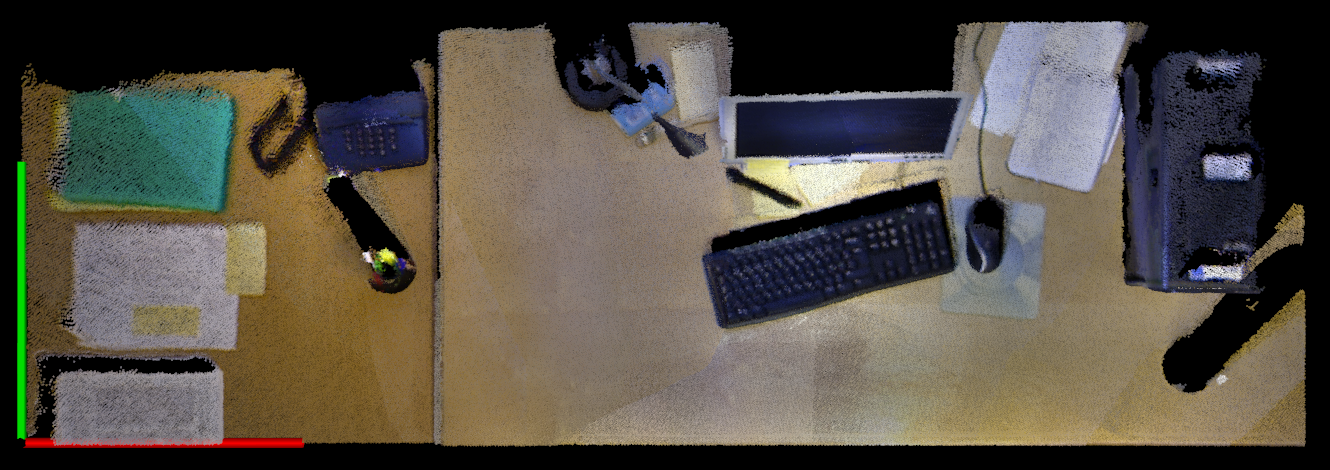
\includegraphics[height=2.5cm]{David_Mor_131110} \quad
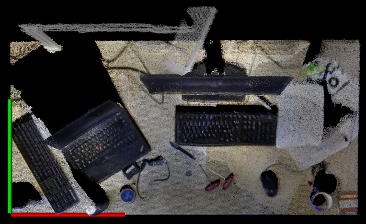
\includegraphics[height=2.5cm]{Nils_Mor_131111} \quad
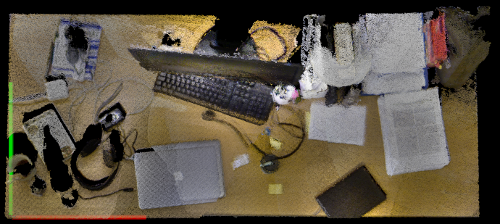
\includegraphics[height=2.5cm]{Puren_Eve_131029}\\ \smallskip
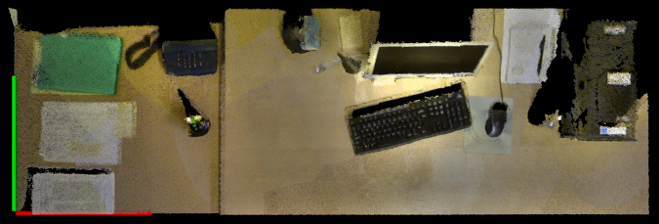
\includegraphics[height=2.5cm]{David_Eve_131110} \enskip
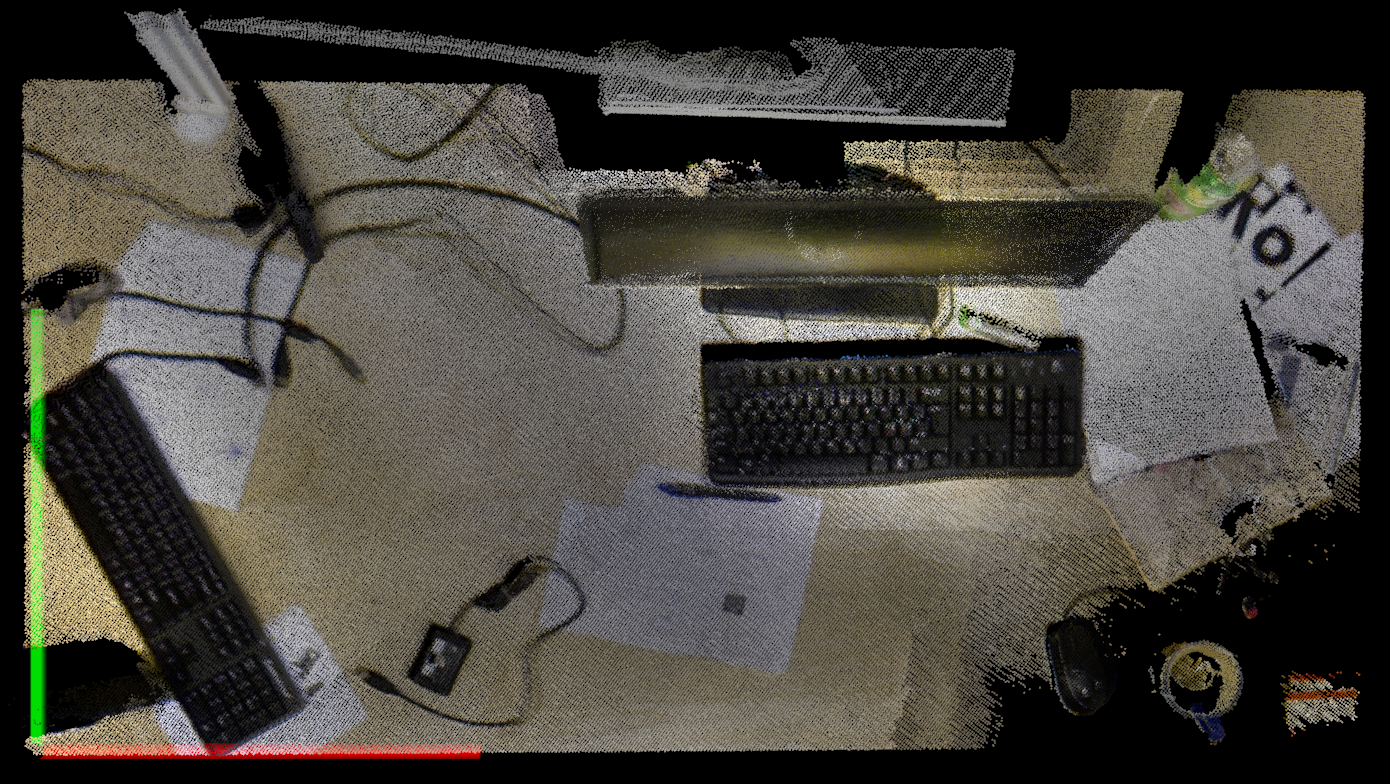
\includegraphics[height=2.5cm]{Nils_Eve_131111} \enskip
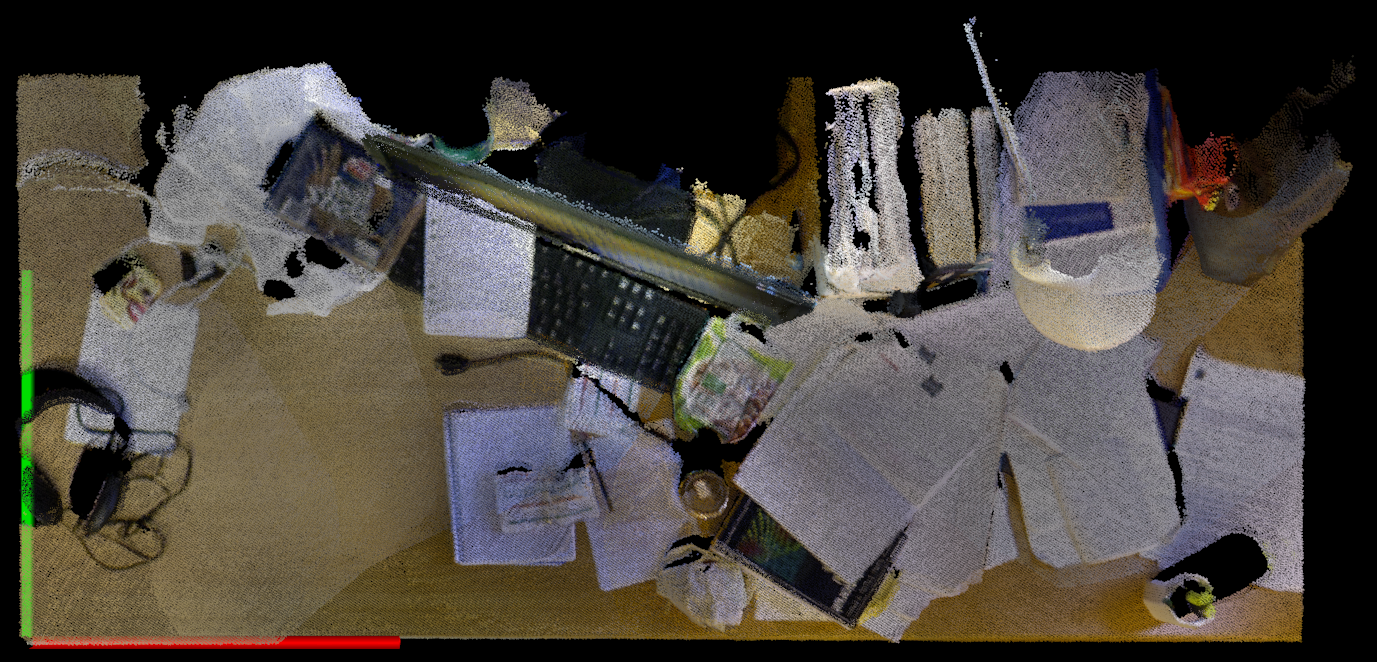
\includegraphics[height=2.5cm]{Puren_Mor_131110}
\label{fig:examplescenes}
\caption{Each column shows a different person's desk. The first two columns show desks in the evening and the morning of the same day whereas the last column shows a desk 12 days apart in time.}
\end{center}
\end{figure*}

Spatial relations have been used previously to provide contextual information to vision-related work. \cite{MyungJin:CVPR2010}used a hierarchy of spatial relations alongside descriptive features to support multiple object detections in a single image. Spatial relations and contextual information are commonly used in activity recognition from video streams. For example, \cite{Krishna:ECAI2010} demonstrate the learning of activity phases in airport videos using spatial relations between tracked objects, and \cite{Behera2012} use spatial relations to monitor objects and activities in videos of a constrained workflow environment. Recent work has used object co-occurrence to provide context in visual  tasks. Examples in 2D include object co-occurrence statistics in class-based image segmentation~\cite{Ladicky:IJCV2013}; and the use of object presence to provide context in activity recognition~\cite{Li:2012}. However, all this previous work is restricted to 2D images, whereas our approaches work with spatial context in 3D (RGB-D) data. Authors have also worked with spatial context in 3D, including parsing a 2D image of a 3D scene into a simulated 3D field before extracting geometric and contextual features between the objects \cite{Xiao:SIGGRAPH2012}. Our approaches to encoding 3D spatial context could be applied in these cases, and we use richer, structured models of object relations.

Apart from using the statistics of co-occurrence, a lot of information can be exploited from \textit{how} the objects co-occur in the scene, i.e. the extrinsic, geometric spatial relations between the objects. Recent work in 3D semantic labelling has used such geometric information along with descriptive intrinsic appearance features~\cite{Koppula:NIPS2011}. They achieve a high classification accuracy for a large set of object-classes belonging to home and office environments. Scene similarity measurement and classification based on contextual information is conducted by \cite{Fisher:ACMT2011}. They also use spatial information for context-based object search using Graph Kernel Methods. The method is further developed to provide synthetic scene examples using spatial relations \cite{Fisher:ACMT2012}. In~\cite{Aydemir:ICRA2011} spatial relations between smaller objects, furniture and locations is used for pruning in object search problems in human environments. In \cite{Lin:ICCV2013} a technique is developed for automatic annotation of 3D objects. It uses intrinsic appearance features and geometric features and is employed to build an object and scene classifier using conditional random fields. In \cite{kasper:2011} the authors utilise both geometric single object features and pair-wise spatial relations between objects to develop an empirical base for scene understanding. Recent studies \cite{Southey:2007,kasper:2011} compute statistics of spatial relations of objects and use it for conditional object recognition for service robotics. Whilst our techniques are comparable to those in the literature, our contribution comes from the explicit comparison of different representations of spatial context (metric vs qualitative) on a novel, long-term learning task. Additionally our qualitative approach relies on relationships which could be provided through other mechanisms than unsupervised machine learning (e.g. through a human tutor describing a spatial scene), and in this way bootstrap the system using expert knowledge.

Our work is evaluated on a new 3D long-term dataset. Other datasets exist: The \textit{B3DO dataset} \cite{Janoch:ICCV2011} which contains many single-snapshot instances of indoor human environments having a variety in viewpoints, object-classes, scene-classes and instances. This dataset is in the form of RGB and depth image pairs with manual 2D annotations of object classes, capturing many unique scenes with the sole aim of finding more realistic scenes which are difficult for PSs to perform scene classification. \textit{NYU Depth V1-2} \cite{Silberman:ECCV2012} datasets contain different instance examples of object-classes and scene-classes. Each image instance is a combo of synchronous RGB and D images of a different scene-class with semantic annotation provided to every pixel. This dataset is aimed at helping PSs with automatic semantic segmentation and scene classification. The \textit{3D IKEA database} \cite{Swadzba:RAS2012} has been collected using robotic maneuvering in different scene-class instances. The aim is to test scene-classification algorithms based on large furniture level objects. The \textit{WRGBD dataset} \cite{Lai:ICRA2011} is aimed to support object classification methods and contains many instances of isolated objects in .pcd format. Annotation is done by assigning every pixel a correct semantic label.None of these datasets contain periodically collected data or easily usable spatial annotations of objects which are key for long-term autonomous scene-learning, based on spatial relations.

The required regularity in instances and time was the main motivation for the construction of this dataset, as currently available datasets either are of individual objects or singular instances of entire rooms

%%%%%%%%%%%%%%%%%%%%%%%%%%%%%%%%%%%%%%%%%%%%%%%%%%%%%%%%%%%%%%%%%%
%%%%%%%%%%%%%%%%%%%%%%%%%%%%%%%%%%%%%%%%%%%%%%%%%%%%%%%%%%%%%%%%%%

%%%%%%%%%%%%%%%%%%%%%%%%%%
%%%%%%%%%%%%%%%%%%%%%%%%%

\begin{enumerate}
  \item More on dataset papers
\end{enumerate}

%%%%%%%%%%%%%%%%%%%%%%%%%%%%%%%%%%%%%%%%%%%%%%%%%%%%%%%%%%%%%%%%%%%%%%%%%%%%%%%%

\section{Motivating Scenario}
\label{sec:Motivating Scenario}

We are investigating systems that operate for long periods of time in environments populated by humans. 
As a motivating scenario we will look at security guard in an office building. The robot patrols the working environment and should learn 
models of what the environment normally looks like and what variations there are. In an implementation of such a system the robot tell when 
something differs from the ordinary too much and then raise an alarm. Initially we will focus on desktop scenes. We are interested in models 
for individual desks and as well as general models of desks. Our working hypotheses is that there is some general rules for how desks are 
organized that we want to be able to extract and later exploit when building the models. We expect that object will change place, within certain semantic bounds. Some objects could be missing at times (coffee mug) which is normal, but some other objects are rarely moved (monitor).

Another aim is to be able to transfer knowledge from one environment to the next. This would allow a robot that just entered a new 
environment to be functional from the start. Concretely this would correspond to having a reasonable prior which can then be adapted when 
new observations are available. What information is general and what is environment specific? How do we represent the knowledge in a way that caters for the knowledge transfer, the ability to learn from few samples and adapting existing models? These are some further examples of questions that we want to study.

To study these questions we need data to learn from. The data need to capture both variations across different desks but also over time. None of the datasets available (see Section~/ref{sec:Related Work}) meet these requirements which is the motivation for the work behind the dataset that we present in this paper.

\subsubsection*{Points Discussed}
\begin{enumerate}
	\item This section should stress why it is important to gather to such datasets
	\item what type of data do we really need? - hint it
	\item reference to related work section to show that this dataset is unique.
\end{enumerate}


%%%%%%%%%%%%%%%%%%%%%%%%%%%%%%%%%%%%%%%%%%%%%%%%%%%%%%%%%%%%%%%%%%%%%%%%%%%%%%%%


\section{Dataset}
\label{sec:Dataset}

Most of the human outdoor and especially indoor environments, are characterized by a supporting surface on which all relevant objects are placed e.g. Land - buildings, living room floor - furniture, dining table - cutlery and dishes etc. It is hence convenient to perceive a structure for the object arrangement in the human environments to be as if on a "nested table-top system". Table-tops are the most commonly present large objects in any floor map. They provide for a favourable prototypical example for analysis of object organization structure. Moreover, it is highly likely that objects on a "table" have more semantic and organizational correlation amidst them, than when compared to those objects not on that same "table" e.g. \textit{Pen} has more semantic/functional correlation with a \textit{Laptop} (on the table) than a \textit{Couch} (not on that table, here the "table" references to the floor of the room).

With the aim of exploring possibilities to understand, learn and model these organizational formalities amongst objects in human indoor environments, a first, pertinent dataset has been composed by periodically capturing observations of entire table-tops of a fixed set of researchers at a computer science research facility called 3D Table-Tops Dataset for Long Term Autonomous Learning. These observations have been made periodically with intervals of few hours, over many days and various instances of object classes. The dataset therefore captures the individual and group variation in object position and pose due to humans and their interaction with the environment. The required regularity in instances and time was the main motivation for the construction of this dataset, as currently available datasets either are of individual objects or singular instances of entire rooms.

%% Blind %%
%KTH University.

It is required for such a long-term autonomous learning to have entire views of the scenes to model the interrelations amidst the member objects. Apart from being variant over object instances across different scenes, the data needed to be periodic over time at a scale of couple of hours so as to capture the individual and group variations in position and pose when there has been regular/irregular human interaction involved. The currently available datasets either are of individual objects or single instances of entire rooms. The required regularity in instances and time was the main motivation for the construction of this dataset (Section~\ref{sec:Related Work}).

\subsection{Dataset Design}

\subsubsection*{Points Discussed}
\begin{enumerate}
	\item Why did we collect it the way we did?
	\item What did we collect?
	\item Time and people level slicings
	\item weekends and weekdays
	\item different times of the day
	\item We want the data to have these properties and hence we designed the dataset in this way.
\end{enumerate}
The target research groups to benefit from this dataset are of the kind that develops artificial intelligence for autonomous robots augmenting human activities (especially if they are fatiguing) within indoor human environments. Hence, it becomes essential for robotic learning to pay attention to variances in human environments wrt. scales of time, space and instances in the same space. The dataset has been composed by capturing and manually annotating 3D images of office type table-tops, for a fixed set of people, at fixed times of the day and for a span of many days.

Observing the table-tops of the same set of people at different times of the day gives insight about the daily interactions a human has with his table and over many days gives an understanding of the gradual variances in their table-top setups. If the data is observed for an entire week, including weekends, features in the table-top configurations, that can be used for estimation of the type of the day of the week, can also be extracted (Weekdays, Fridays, Weekends). Table-top models can also be learnt for all the people put together -- which gives a gross functional representation of a typical table-top in general for research employees in office environments -- or for individual people which helps to gain functional representations of office table-tops for individuals, seniority, gender and so on. Finally, when trying to find general models over any of these types of data partition, the model learns to be able to generalize over different instances of a fixed set of object classes. In summary: When the dataset is partitioned in different ways with respect to time, people or instances, it richly yields knowledge and hence representations of table-tops in office environments.

As explained in Section~\ref{sec:Motivating Scenario} our research intentions are to provide intelligence to an long-term operating, autonomous, human activity augmenting robot for indoor human environments. The concept of composing the 3D-TOTAL dataset follows naturally from this research motivation.

The dataset is a collection of human-annotated office table scenes from a computer science research institute. The data was collected using the \textit{SCENECT} software \cite{Buerkler:Online2012} and an \textit{Asus Xtion Pro} RGB-D camera. Within the data, a \textit{Scene} is defined to be a single instance of a table-top of one person at a single instance in time. There is one 3D colour point cloud per scene (.pcd format). Every scene is a reconstructed version of the raw data stream obtained by a person scanning a table-top with real time visual feedback using SCENECT. The software has in-built real-time sampling, registration and de-noising algorithms to output the final high resolution point cloud.

The scenes were recorded as periodically as possible and at three fixed time instances of the day: \emph{Morning} (09:00 hrs), \emph{Afternoon} (13:00 hrs) and \emph{Evening} (18:00 hrs). Scenes for 20 different tables were collected for 19 days, 3 times per day. A \textit{Scene\_ID} is attached to each scene to indicate who the table belongs to and the date and time of the recording. These Scene\_IDs help in slicing across the dataset with respect to time of the day \{Morning, Afternoon, Evening\}, person \{Anna, Bob, Carl, \dots\}, or day \{2013-11-01, 2013-11-06, 2013-11-13, \dots\}.

A 3D annotation tool was developed for manually segmenting out objects of interest from the point clouds. On average, 12 different objects were labelled per scene. The objects belong to the following super set - \{Mouse, Keyboard, Monitor, Laptop, Cellphone, Keys, Headphones, Telephone, Pencil, Eraser, Notebook, Papers,  Book, Pen, Highlighter, Marker, Folder, Pen-Stand, Lamp, Mug, Flask, Glass, Jug, Bottle\}. The information about every scene and object is available in  XML and JSON formats. Each scene has a nested list of object data containing \{Position, Orientation, Size, Date and Time of recording, Person ID, Point Indices of the point cloud that have been labelled as belonging to the Object\}.

\subsection{Dataset Realization}
A 3D dataset " \textit{Tables for Spatial Modelling}" has been created by KTH, Royal Institute of Technology. The dataset is a collection of human annotated office tables of researchers at KTH. This is the ground truth data to train models for spatial configuration of Office Tables.

The data was collected using a freely available software called \textit{SCENECT} \cite{} and an \textit{Asus Xtion Pro} RGB-D camera. A \textit{Scene} is defined to be a single instance of a table-top of one person at one time instance. There is one 3D colour image in the form of a point cloud per scene (.pcl format). Every scene is a reconstructed version of the raw data stream obtained by a person scanning a table-top with real time visual feedback using SCENECT. The software has in-built real-time sampling, registration and de-noising algorithms to output the final high resolution point cloud.

The scenes were recorded as periodically as possible and at three fixed time instances of the day: Morning (09:00 hrs), Afternoon (13:00 hrs)and Evening (18:00 hrs). The scenes were collected for 19 days, 3 times per day and for the same 20 different tables. Depending on who the table belongs to and the date and time of the recording, each table-top scene recording receives a \textit{Scene\_ID}. These Scene\_IDs help in slicing across the dataset with respect to time of the day \{Morning, Afternoon, Evening\}, or people\{Akshaya, Yuquan, Carl,...\}, or day \{2013-11-01, 2013-11-06, 2013-11-13,...\}.

A \textit{3D Annotation Tool} was developed at KTH for manually segmenting out objects of interest from the point clouds. On an average 12 different objects were labelled per scene. The objects belong to the following super set - \{Mouse, Keyboard, Monitor, Laptop, Mobile, Keys, Headphones, Telephone, Pencil, Rubber, Notebook, Papers,  Book, Pen, Highlighter, Marker, Folder, Pen-Stand, Lamp, Mug, Flask, Glass, Jug, Bottle\}. The information about every scene and each object are available in the .xml and .json formats. Each scene data has a nested list of object data, and each object data has the following information about the object - \{Position, Orientation, Size, Date and Time of recording, Person ID, Point Indices of the point cloud that have been labelled as belonging to the Object\}.
\subsubsection*{Points Discussed}
\begin{enumerate}
	\item Annotation Tool
	\item Tools for collecting Asus Scenect
	\item 
\end{enumerate}

\subsection{Dataset Summary}
\begin{enumerate}
	\item Dataset details - days, objects, people, times
	\item \textbf{figure} showing variations over different times of day, different people
	\item details of XML and JSON files
	\item \textbf{figure} Histograms of object occurrences
\end{enumerate}

\begin{figure}[t]
\begin{center}
\subfloat[][]{\label{fig:HistOfObjects}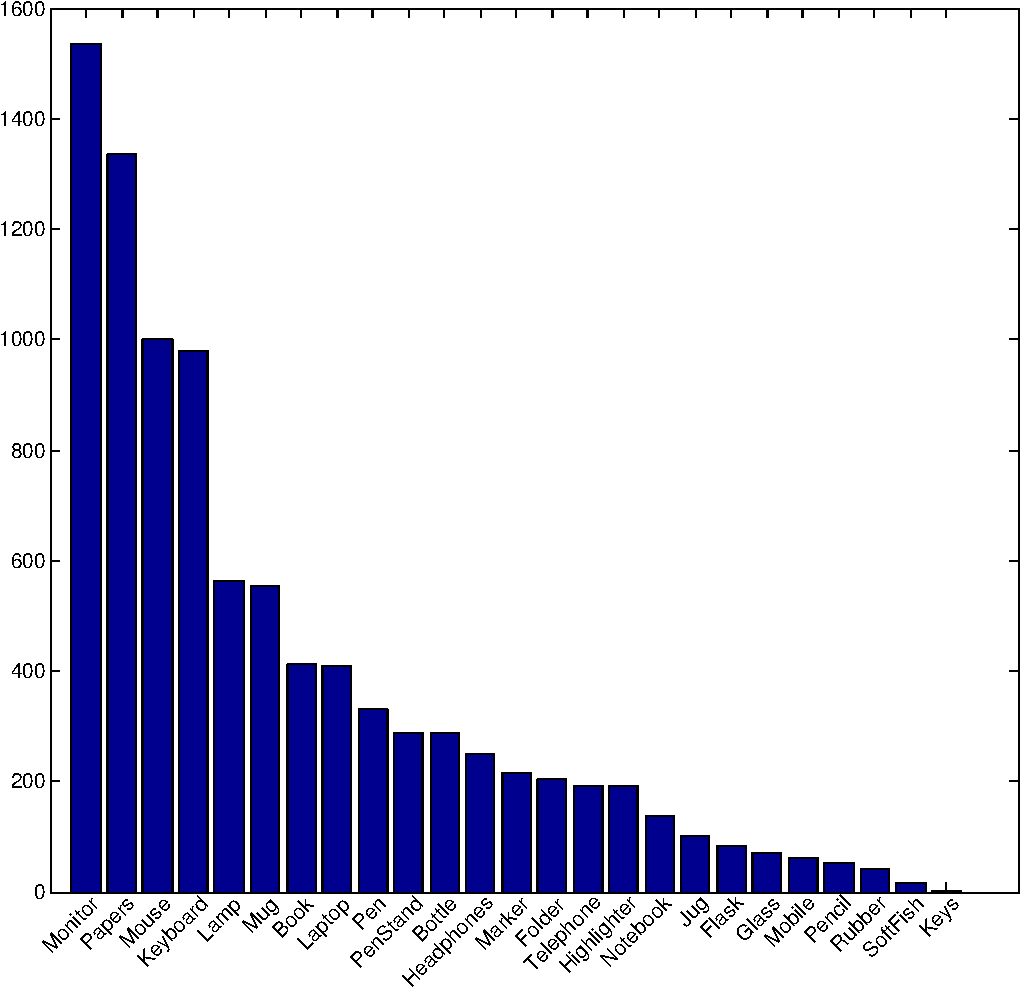
\includegraphics[width=0.8\linewidth]{HistOfObjects_crp.pdf}}\\
\subfloat[][]{\label{fig:RawPCD}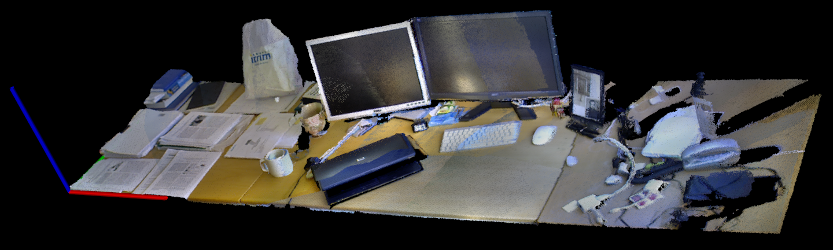
\includegraphics[width=0.7\linewidth]{pcd.png}}\\
\subfloat[][]{\label{fig:RawPCDAnnotated}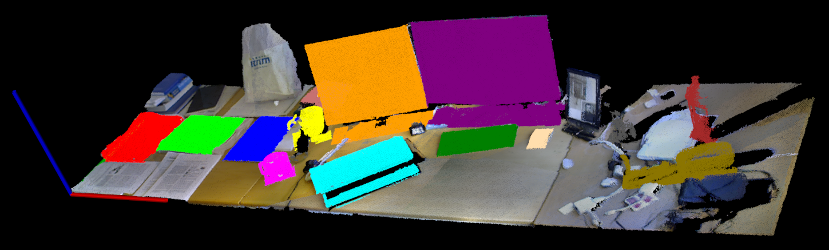
\includegraphics[width=0.7\linewidth]{pcd_annotated.png}}
\caption{(a) Objects annotated in 3D Long-Term Dataset, sorted in descending order of count of occurrences. X-axis$=$Object Name, Y-axis$=$Occurrence Count. (b) Screenshot of one table scene, along with it's annotations in (c).}

\end{center}
\end{figure}


%%%%%%%%%%%%%%%%%%%%%%%%%%%%%%%%%%%%%%%%%%%%%%%%%%%%%%%%%%%%%%%%%%%%%%%%%%%%%%%%

\section{Analysis}
\label{sec:Analysis}

\begin{itemize}	
\item keyboard
\item monitor
\item mouse
\item mug
\item laptop
\item papers
\item book
\item bottle
\item jug
\item notebook
\item mobile
\item glass
\item flask
\end{itemize}

%\begin{figure}
%\begin{tabular}{ccc}
%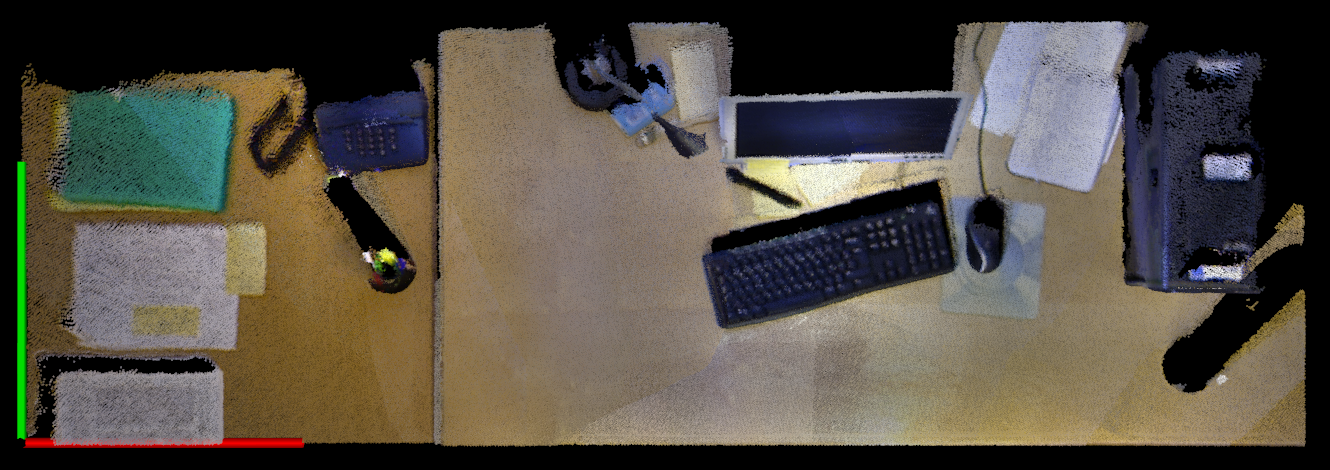
\includegraphics[height=2.5cm]{David_Mor_131110}&
%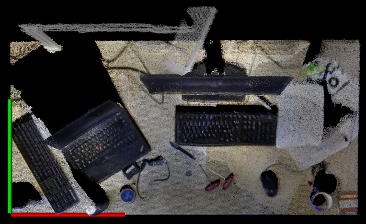
\includegraphics[height=2.5cm]{Nils_Mor_131111}&
%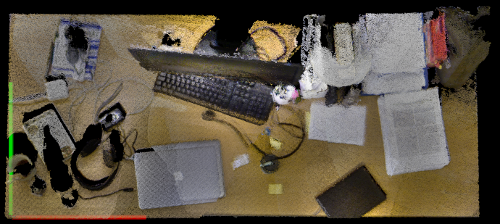
\includegraphics[height=2.5cm]{Puren_Eve_131029}\\
%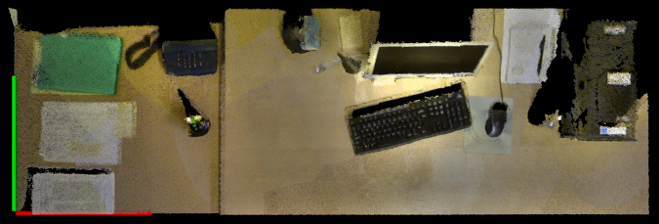
\includegraphics[height=2.5cm]{David_Eve_131110}&
%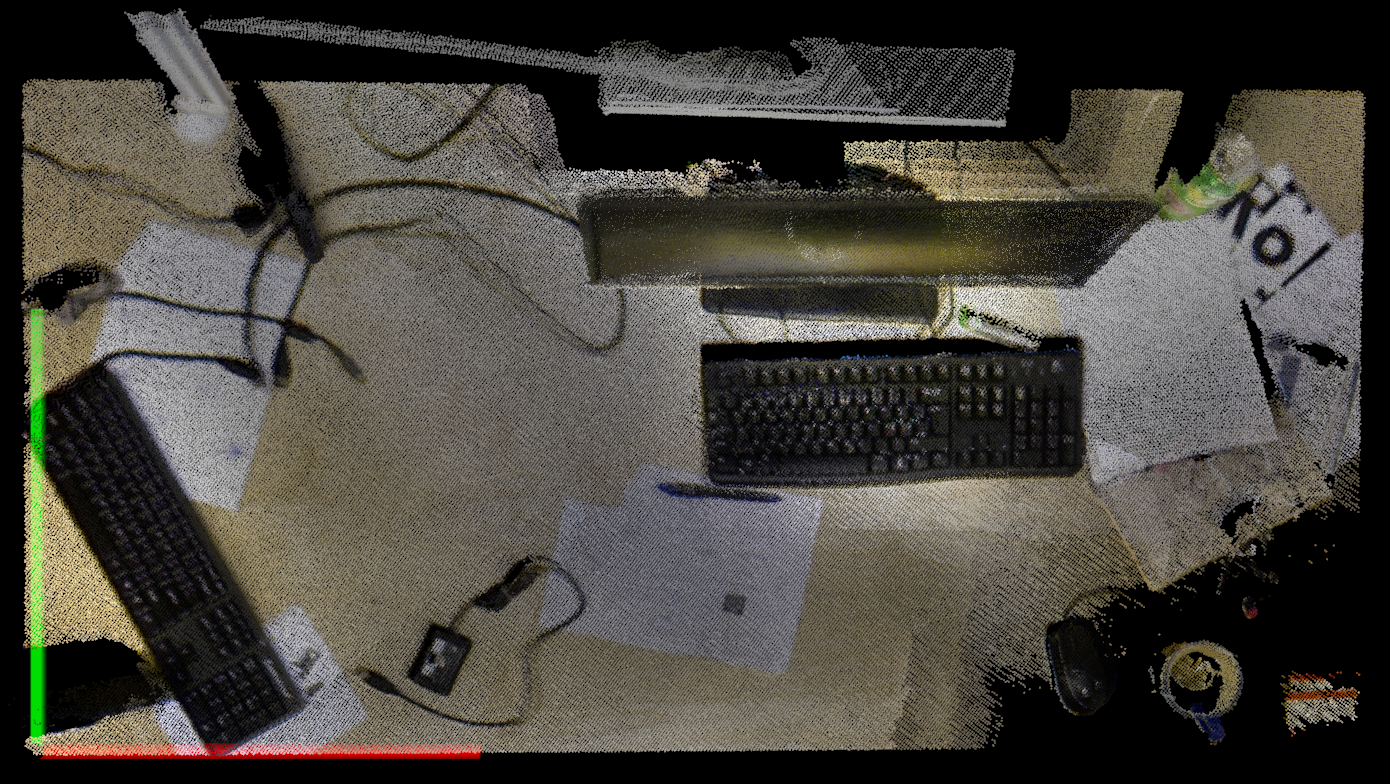
\includegraphics[height=2.5cm]{Nils_Eve_131111}&
%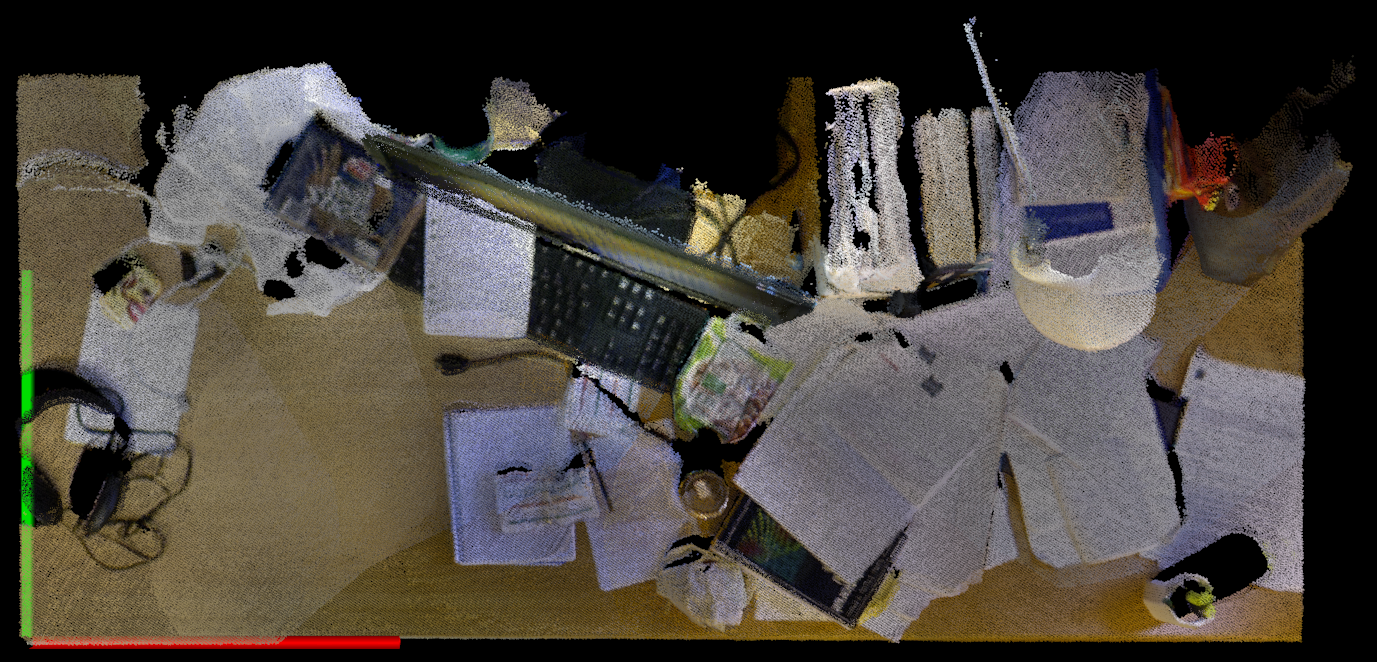
\includegraphics[height=2.5cm]{Puren_Mor_131110}
%\end{tabular}
%\label{fig:examplescenes}
%\caption{Each column shows a different person's desk. The first two columns show desks in the evening and the morning of the same day whereas the last column shows a desk 12 days apart in time.}
%\end{figure}



\begin{figure}
\begin{center}
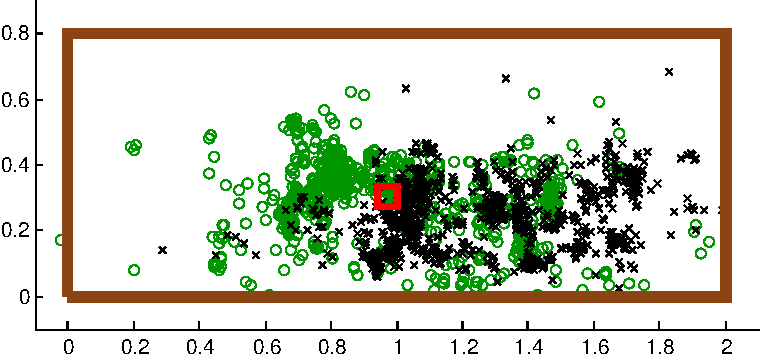
\includegraphics[width=0.8\linewidth]{keyboard_mouse_raw-crop}
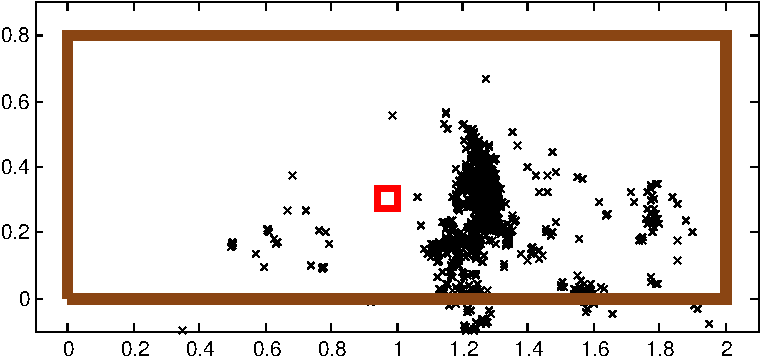
\includegraphics[width=0.8\linewidth]{keyboard_mouse-crop}
\end{center}
\label{fig:scatter-keyboard-mouse}
\caption{This figure investigates the correlation in position of keyboard and mouse. Top: The green circles shows the position of the centroid of each keyboard that exist in a scene where there is at least one mouse. The black crosses show the position of all mice in scenes with at least one keyboard. The red square shows the mean position of all keyboards. Bottom: By shifting the position of keyboard and mouse such that the keyboards are at the mean keyboard position we can illustrate the position of the mouse relative to the keyboard. As expected most mice are to the right of the keyboard.} 
\end{figure}

\begin{figure}
\begin{center}
\subfloat[][]{\label{fig:scatter-monitor-keyboard}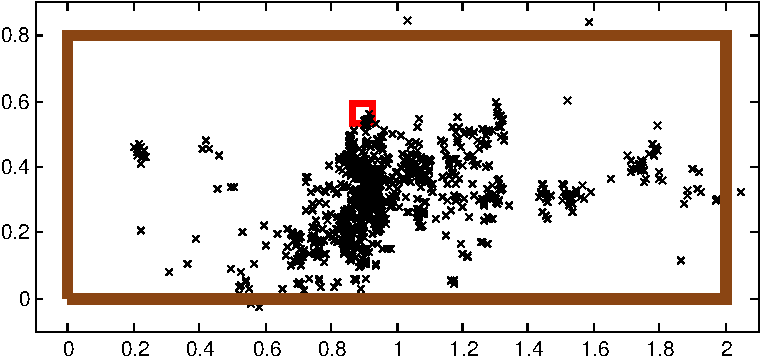
\includegraphics[width=0.8\linewidth]{monitor_keyboard-crop}}\quad
\subfloat[][]{\label{fig:scatter-keyboard-mug}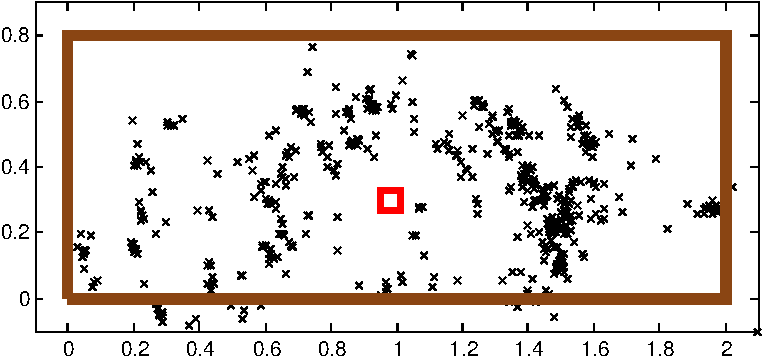
\includegraphics[width=0.8\linewidth]{keyboard_mug-crop}}\\
\subfloat[][]{\label{fig:scatter-keyboard-papers}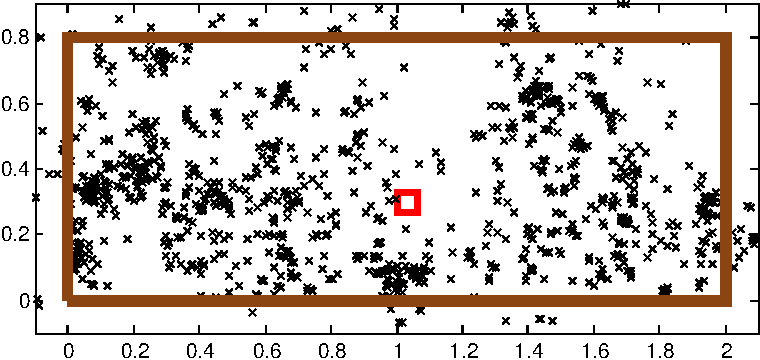
\includegraphics[width=0.8\linewidth]{keyboard_papers-crop}}
\end{center}
\label{fig:scatter-rest}
\caption{The figures show the relative position of a) keyboard w.r.t. monitor, b) mug w.r.t. keyboard and c) papers w.r.t. keyboard. Qualitatively keyboards are mostly infront of monitors, mugs are around the keyboard and the position of papers is mostly independent on the position of the keyboard.} 
\end{figure}


\begin{table*}
\begin{center}
\begin{tabular}{|l||c|c|c|c|c|c|c|c|c|c|c|c|c|}
\hline
& $C_{1}$ & $C_{2}$ & $C_{3}$ & $C_{4}$ & $C_{5}$ & $C_{6}$ & $C_{7}$ & $C_{8}$ & $C_{9}$ & $C_{10}$ & $C_{11}$ & $C_{12}$ & $C_{13}$\\ \hline \hline
$C_1$: Keyboard & 0.76 & 3.54 & 2.79 & 4.01 & 3.56 & 4.57 & 4.00 & 3.78 & 3.11 & 3.18 & 2.78 & 3.25 & 2.95 \\ \hline
$C_2$: Monitor & 3.41 & 1.65 & 3.35 & 4.06 & 3.39 & 4.63 & 4.19 & 3.86 & 3.48 & 3.16 & 3.01 & 3.37 & 2.95 \\ \hline
$C_3$: Mouse & 2.89 & 3.59 & 0.73 & 3.81 & 3.59 & 4.56 & 3.96 & 3.84 & 3.30 & 3.09 & 3.02 & 3.27 & 2.93 \\ \hline
$C_4$: Mug & 4.08 & 4.21 & 3.71 & 0.74 & 3.67 & 4.47 & 3.99 & 3.73 & 2.85 & 2.78 & 3.06 & 3.17 & 3.08 \\ \hline
$C_5$: Laptop & 3.79 & 3.60 & 3.67 & 3.70 & 0.05 & 4.34 & 3.67 & 3.23 & 3.09 & 2.86 & 2.69 & 3.30 & 2.47 \\ \hline
$C_6$: Papers & 4.45 & 4.50 & 4.22 & 4.41 & 4.01 & 2.76 & 4.30 & 3.84 & 3.41 & 3.49 & 3.29 & 3.72 & 3.36 \\ \hline
$C_7$: Book & 3.96 & 3.93 & 3.81 & 3.86 & 3.67 & 4.49 & 0.77 & 3.42 & 2.76 & 2.93 & 2.59 & 3.35 & 2.81 \\ \hline
$C_8$: Notebook & 3.90 & 3.99 & 3.68 & 3.70 & 3.29 & 4.16 & 3.59 & 0.28 & 1.83 & 2.40 & 1.81 & 2.62 & 1.97 \\ \hline
$C_9$: Mobile & 3.37 & 3.50 & 3.30 & 3.09 & 3.19 & 3.79 & 3.13 & 1.83 & 0.00 & 1.91 & 1.75 & 2.28 & 1.28 \\ \hline
$C_{10}$: Glass & 3.46 & 3.60 & 3.28 & 2.89 & 3.05 & 3.96 & 2.70 & 2.04 & 2.08 & 0.41 & 2.15 & 2.57 & 1.35 \\ \hline
$C_{11}$: Flask & 2.98 & 3.28 & 3.22 & 3.13 & 2.87 & 3.68 & 2.88 & 2.06 & 1.75 & 2.20 & 0.00 & 2.80 & 1.44 \\ \hline
$C_{12}$: Bottle & 3.47 & 3.64 & 3.44 & 3.42 & 3.17 & 4.03 & 3.33 & 2.58 & 2.55 & 2.45 & 2.77 & 1.03 & 2.74 \\ \hline
$C_{13}$: Jug & 3.05 & 3.34 & 2.85 & 3.11 & 2.54 & 3.56 & 2.81 & 1.97 & 1.28 & 1.55 & 1.43 & 2.95 & 0.00 \\ \hline
\end{tabular}
\label{fig:entropy}
\caption{The table shows the entropy in the spread in positions that results when looking at the position of one object (columns) with respect to that of another one (rows). As we can see papers have high entropy in combination with all other objects which indicates that the distribution of relative positions is close to uniform. Other combinations such as Keyboard and Mouse have much lower entropy, that is, more peaky distribution showing a stronger correlation.}
\end{center}
\end{table*}

\subsubsection*{Points Discussed}
\begin{enumerate}
	\item \textbf{figure} Scatter plot for variation within person ID
	\item \textbf{figure} Scatter plot for variation wrt object type
	\item \textbf{figure} Scatter plot for variation considering different landmark - trajectors.
	\item \textbf{figure} Scatter plot of 2D footprints of objects
	\item General conclusions about above figures.
	\item 
	\item 
\end{enumerate}

%%%%%%%%%%%%%%%%%%%%%%%%%%%%%%%%%%%%%%%%%%%%%%%%%%%%%%%%%%%%%%%%%%%%%%%%%%%%%%%%
\section{Conclusions}
\label{sec:Conclusions}

%%%%%%%%%%%%%%%%%%%%%%%%%%%%%%%%%%%%%%%%%%%%%%%%%%%%%%%%%%%%%%%%%%%%%%%%%%%%%%%%
\section{Future Work}
\label{sec:Future Work}

%%%%%%%%%%%%%%%%%%%%%%%%%%%%%%%%%%%%%%%%%%%%%%%%%%%%%%%%%%%%%%%%%%%%%%%%%%%%%%%%
\subsubsection*{Points Discussed}
\begin{enumerate}
	\item Room level data set
	\item Which QSR for which purpose?
\end{enumerate}

%%%%%%%%%%%%%%%%%%%%%%%%%%%%%%%%%%%%%%%%%%%%%%%%%%%%%%%%%%%%%%%%%%%%%%%%%%%%%%%%
\section{Acknowledgements}
\label{sec:Acknowledgements}
CVAP-KTH, Accel Partners, STRANDS project

\bibliographystyle{ieeetr}
\bibliography{references}

\end{document}